\documentclass{ctexart}
\usepackage{amsmath}
\usepackage{amssymb}
\usepackage{graphicx}
\usepackage{gbt7714}
\usepackage{wrapfig}
\ctexset{
    % 修改 section。
    section={   
        name={,、},
        number={\chinese{section}}
    }
}

\title{在气垫导轨上研究简谐振动}
\author{陆知辰-10225301456}
\date{\today}
\graphicspath{{figure/}}

\begin{document}

\begin{titlepage}
  \centering
  % 插入图片
  
\includegraphics[width=0.5\textwidth]{ecnu.png}
  
  % 空行用于调整标题位置
  \vspace*{\baselineskip}
  
  % 标题
  \Huge\textbf{物\quad 理\quad 实\quad 验 \quad (二)}
  % 空行用于调整标题和其他信息之间的间距
  \vspace*{0.3\baselineskip}
  
  % 具体实验名称
  \huge 在气垫导轨上研究简谐振动
  
  % 空行用于调整时间和其他信息之间的间距
  \vspace*{2\baselineskip}
  
  % 时间
  \large 时间:\today
  
  % 空行用于调整时间和其他信息之间的间距
  \vspace*{\baselineskip}
  
  % 创作人
  \large 创作人:陆知辰
  
  % 空行用于调整创作人和学号之间的间距
  \vspace*{\baselineskip}
  
  % 学号
  \large 学号:10225301478
  
\end{titlepage}
\newpage
\tableofcontents
\newpage
\section{实验摘要}
  \subsection{实验概要}
  简谐振动是周期运动中最简单的运动方式。研究简谐振动是了解周期运动最简单最理想的模型。对于简谐振动而言,
  其动力学特征是受力情况满足$F=-kx$。其中$x$为偏离平衡位置的位移大小。
  本实验就是在气垫导轨上研究简谐子在简谐振动的时候的主要特征及其运动形式。
  \subsection{实验目的}
  1.\quad 了解简谐振动运动规律的验证方法及要求。

  2.\quad 了解简谐振动过程中的机械能守恒定律的验证方式。
  
  3.\quad 掌握对数据对结果图形的处理方式。

\section{实验原理}
  \begin{figure}[b]
    \centering
    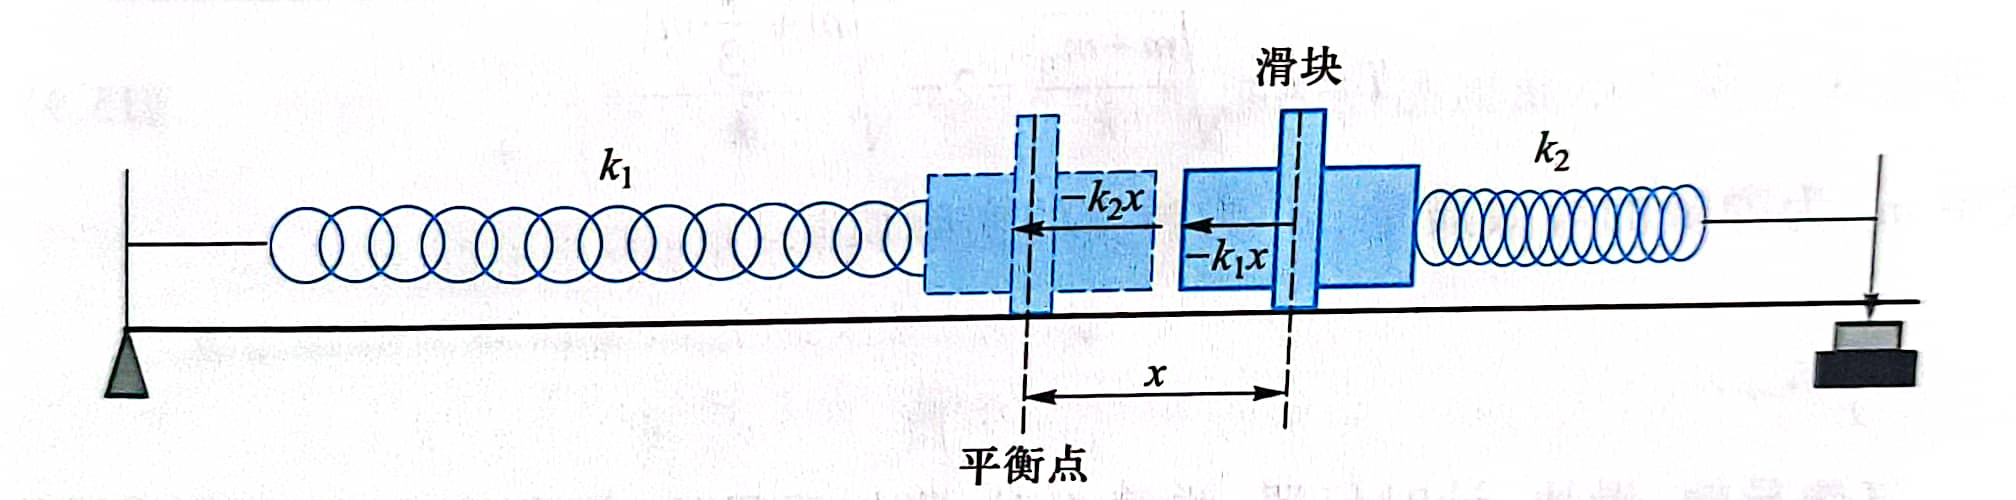
\includegraphics[height=0.3\textwidth,width=1\textwidth]{yuanli1.jpg}
    \caption{实验原理辅助用图}\label{figureyuanli1}
  \end{figure}
在如图\ref{figureyuanli1}中所展示的那样,实验器材的原理可以抽象为如图的模型。装置为一个水平的气垫导轨,不同
弹性系数的弹簧$k_{1}$和$k_{2}$各自的一端固定在两端的支架上,另一端固定在两弹簧中间的质量块上。在滑块静止后拉
动滑块使得滑块偏离平衡位置使弹簧产生弹性形变对滑块有拉力作用。对滑块进行受力分析可得当滑块偏离平衡位置的位移
为$x$的时候,所受到的回复力为
\begin{equation}
  F==(k_{1}+k_{2})x
\end{equation}
具体可以将两个弹簧视为一个整体,整体弹簧的弹性系数等于两个分弹簧的弹性系数的和即$k_{和}=k_{1}+k_{2}$。
根据上文对简谐运动特征的分析可以得出该滑块的运动是简谐运动。
这样的近似忽略了空气阻力以及其他形式的能量的损耗。以此为假设就能得出滑块就可以看作一个简谐振动子。

再根据牛顿第二定律$\ddot{a}*m=F$可以列出该滑块的动力学微分方程
\begin{equation}\label{niuerweifengfangchen}
  m\frac{d^2 y}{d x^2}=-kx 
\end{equation}
将方程解出可以得到解为
\begin{equation}\label{weiyifangchenjie}
  x=A\sin \left( \omega t+ {\varphi}_{0} \right)
\end{equation}
对于方程\ref{weiyifangchenjie}而言,式子中的$A$为振幅,${\varphi}_{0}$为初相位,
这两个量只和初始状态有关,是常数。$\omega$为振动频率,和初始状态无关,和系统本身的特征有关。
具体而言,$\omega = \sqrt{\frac{k}{m}} $,所以$\omega$只和$m$与$k$有关。并且两者都是常数。
由此通过$T=\frac{2\pi}{\omega}$可以得出振子的周期还可以表示为
\begin{equation}\label{zhouqiwutanhuang}
  T=2\pi \sqrt{\frac{m}{k}}
\end{equation}
但是上述过程中没有讨论弹簧自身的质量的影响,重新考虑弹簧自身的质量后\ref{zhouqiwutanhuang}式将改写为
\begin{equation}\label{zhouqitanhuang}
  T=2\pi \sqrt{\frac{m+m_{0}}{k}}=2\pi \sqrt{\frac{m+\frac{1}{3}m_{s}}{k}}
\end{equation}
其中\ref{zhouqitanhuang}式中的$m_{0}$为弹簧的等效质量,$m_{s}$为弹簧的实际质量。

已知以上条件后就可以推导出下列的式子

根据\ref{weiyifangchenjie}式可以得出速度的表达式为
\begin{equation}
  v=\frac{dx}{dt} =\omega A \cos \left( \omega t + {\varphi}_{0} \right)
\end{equation}

滑块的动能和振动势能为
\begin{equation}
  E_{k}=\frac{1}{2} mv^{2}=\frac{1}{2}kA^{2} {\cos}^{2}\left( \omega t + {\varphi}_{0} \right)
\end{equation}
\begin{equation}
  E_{P}=\frac{1}{2}kx^{2}=\frac{1}{2}kA^{2} {\sin}^{2} \left( \omega t + {\varphi}_{0} \right)
\end{equation}

最终可以得到总能量为
\begin{equation}
  E=E_{k}+E_{P}=\frac{1}{2}kA^{2}
\end{equation}

\section{实验装置器材介绍}
气垫导轨,滑块,计时仪器,弹簧数对,重物质量块,物理天平,米尺,
若干挡光片。

\section{实验内容及实验步骤}
  \subsection{系统调节}
  安装完光电门传感器后测试光电门计时功能是否正常使用再进行导轨水平调整。
  导轨的水平调节通过导轨一端安装的调节螺丝,用于调节导轨横向与纵向的水平。
  在调节水平的时候通过结合静态调节和动态调节的方式进行调节。
    \subsubsection{静态调节}
    打开气源开关,将滑块放于导轨任意位置,观察滑块是否会发生滑动。反复多次
    调节底部螺丝,直到滑块保持不动,或稍有移动但无一定方向性为止。应选择多个
    位置进行试验。
    \subsubsection{动态调节}
    原理是如果滑块已经调平,则通过导轨任意位置的速度应该相同,滑块作匀速直线
    运动。所以在滑块通过两个光电门的时候的速度应该是相等的。所以以一定初速度
    释放滑块记录滑块通过两个光电门的速度大小并作出相应的调节,最终使得滑块通过
    两光电门的速度相差不超过5\%。
  \subsection{弹簧弹力系数测量}
  测量弹簧原本长度,在悬挂质量块后再次测量长度,多次悬挂不同质量的重物测量弹簧的型变量,通过计算得到
  弹簧的弹性系数。导轨弹簧弹性系数等于两侧弹簧弹性系数的和,即$k_{\mbox{总}}=k_{1}+k_{2}$。
  \subsection{测量x-t数据并验证位移方程}
  记录滑块开始运动为起点,挡光片前后按照运动方向规定,即向右运动则挡光片右侧边为前沿,反之亦然。让滑块在
  导轨自由振动直到停下,此时挡光片前侧为平衡位置,也就是光电门$I$所在位置。

  随后拉动滑块向挡光片后方运动,拉动的位置为$A_{0}$,为初振幅,应该满足$A_{0}>0.2m$。此处规定为实验中每次
  释放滑块的初始位置,标记记号以便之后查找。
  \begin{figure}[h]
    \centering
    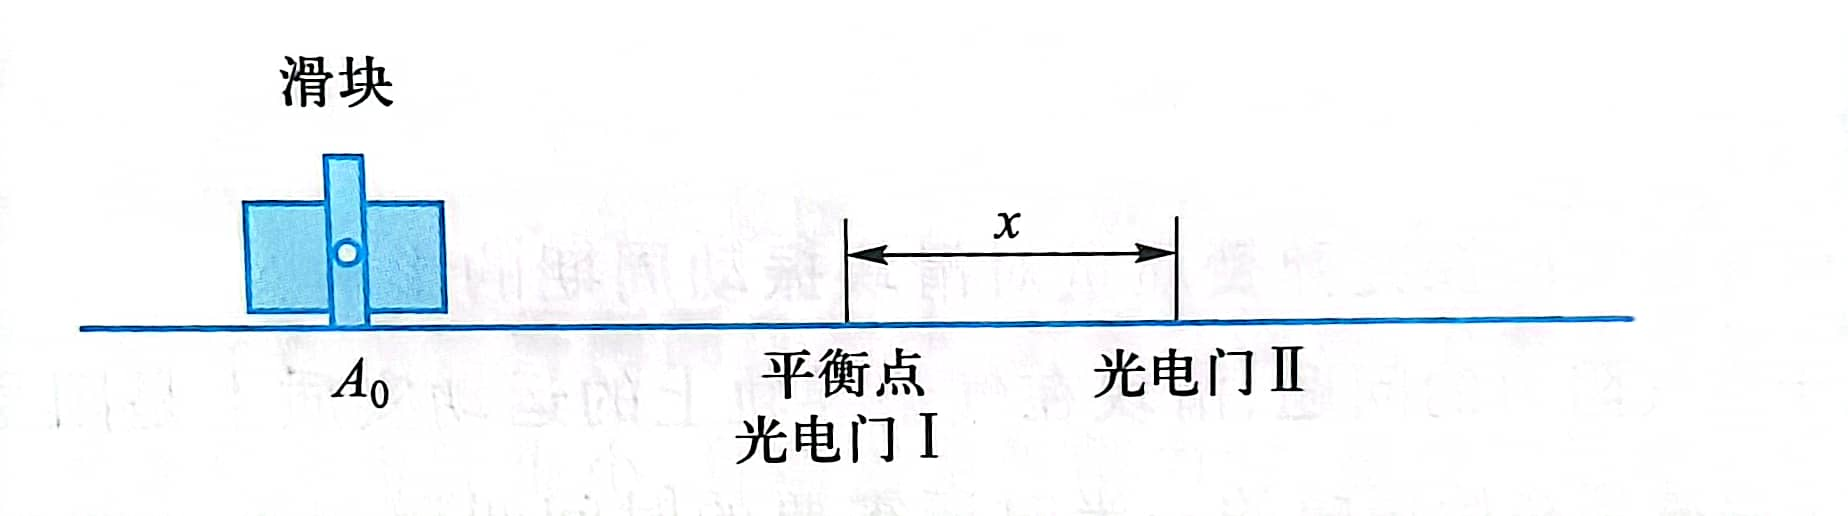
\includegraphics[height=0.3\textwidth,width=1\textwidth]{guangdianmenhuagui.jpg}
    \caption{光电门与滑块位置关系示意图}\label{figureweizhi}
  \end{figure}

  图\ref{figureweizhi}展示的是实验中光电门$I$、光电门$II$和滑块初始位置的关系。光电门$II$的位置为距离
  平衡位置$x$的地方。实验中需要记录滑块从$A_{0}$处释放后从平衡位置运动到$x$处所需要的时间t。
  随后改变x的大小,也就是改变偏离平衡位置的距离,每次改变距离需要等间距并且改变次数不能少于5次。每次实验
  都需要记录$x$位置与所用的时间$t$。

  如果想测量从平衡位置运动到最大位移$A_{0}$处的时间,可以通过先测周期$T$,再计算$\frac{1}{4}T$得出所需时间。
  
  最后还需要对数据进行处理。利用实验中记录的$x-t$数据,在$\frac{1}{4}$个周期内绘制$x-\sin{\omega t}$的图像,将得到
  的斜率和原本的$A_{0}$进行比较,得出结论。

  \subsection{验证振动周期与初始状态无关}
  初始状态包括两部分:初相位与初振幅。所以验证实验也需要控制变量从两个方面进行验证。
    \subsubsection{验证振动周期与初振幅无关}
    将光电门固定在平衡位置,多次改变滑块释放的位置,也就使得初振幅不同,测量滑块的周期。
    \subsubsection{验证振动周期与初相位无关}
    将滑块释放的位置固定,也就是固定初振幅,多次改变光电门所在位置,也就使得初相位不同,测量滑块周期。

  \subsection{验证周期公式$T=2\pi \sqrt{\frac{m}{k}}$}
  将一个光电门放于平衡位置固定,固定初振幅,利用不同的弹簧和不同质量的滑块来改变$\frac{m}{k}$的值,并测量不同情况下的周期。

  进行数据处理的时候希望能够得到线性的关系,对于$T=2\pi \sqrt{\frac{m}{k}}$进行取对数的操作,最终获得式\ref{zhouqibianxing}
  \begin{equation}\label{zhouqibianxing}
    \ln T = \ln 2\pi +\frac{1}{2} \ln \frac{m}{k}
  \end{equation}
  从式中就能获得一组线性关系的变量$\ln T \mbox{和} \ln \frac{m}{k}$。由此可以通过数据处理的方式求出两者线性关系的斜率
  b以及$\ln T$轴的截距,并和理论值进行比较。
\newpage

\section{实验原始数据}
\begin{figure}[h]
  \centering
  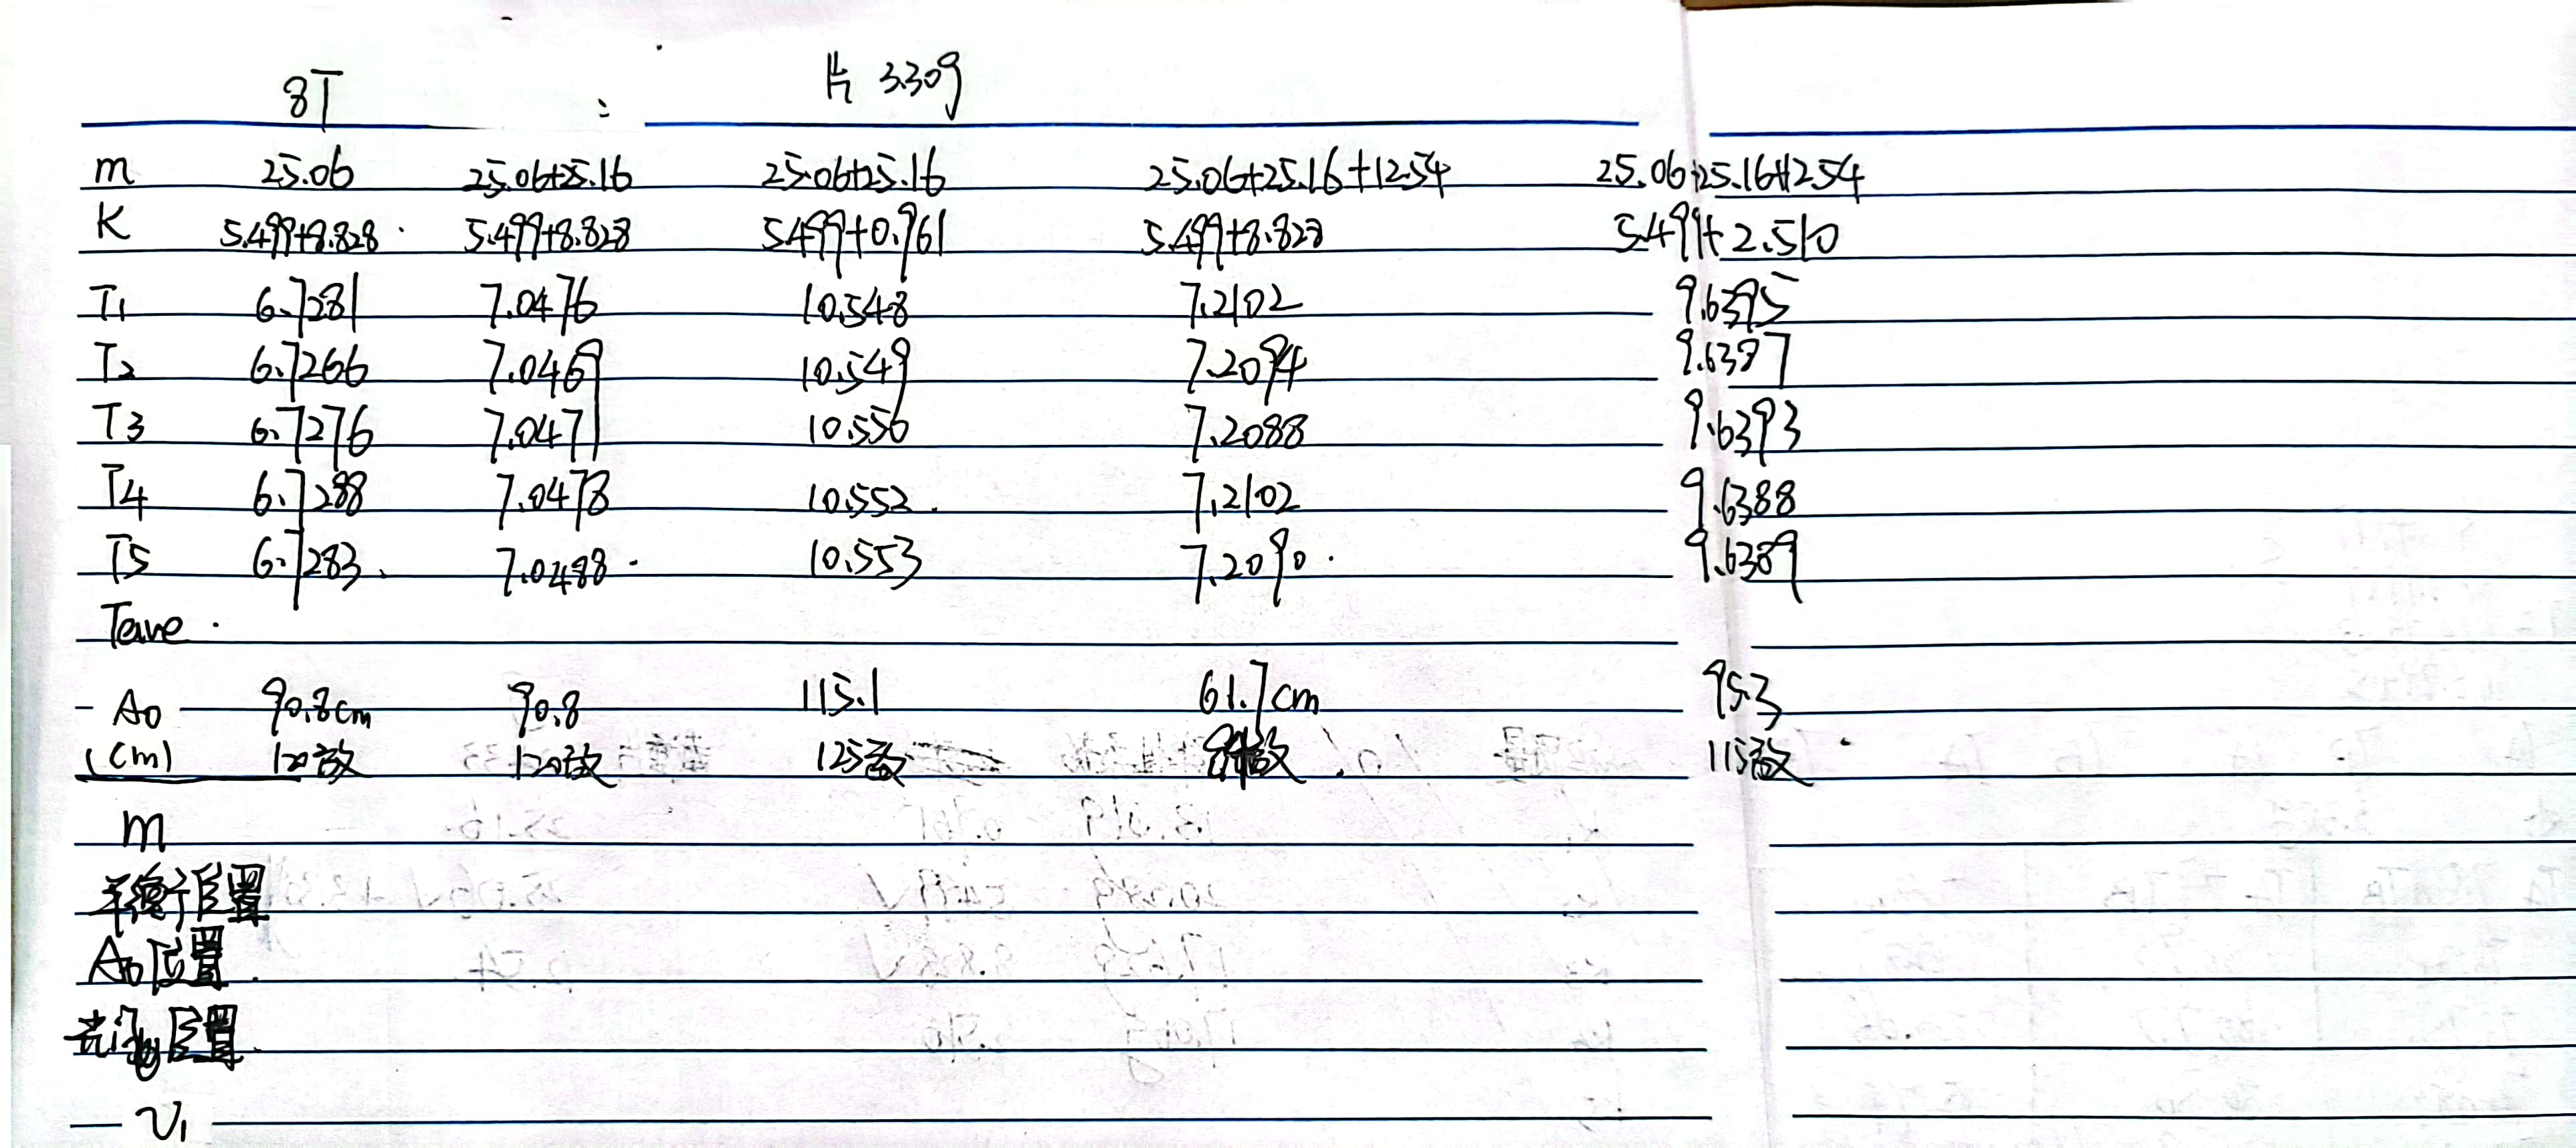
\includegraphics[width=1\textwidth]{yuanshishujv1.jpg}
  \caption{实验原理辅助用图}\label{yuanshishujv1}
\end{figure}
\newpage
%----------------------------------------------------------------------------
\begin{figure}[h]
  \centering
  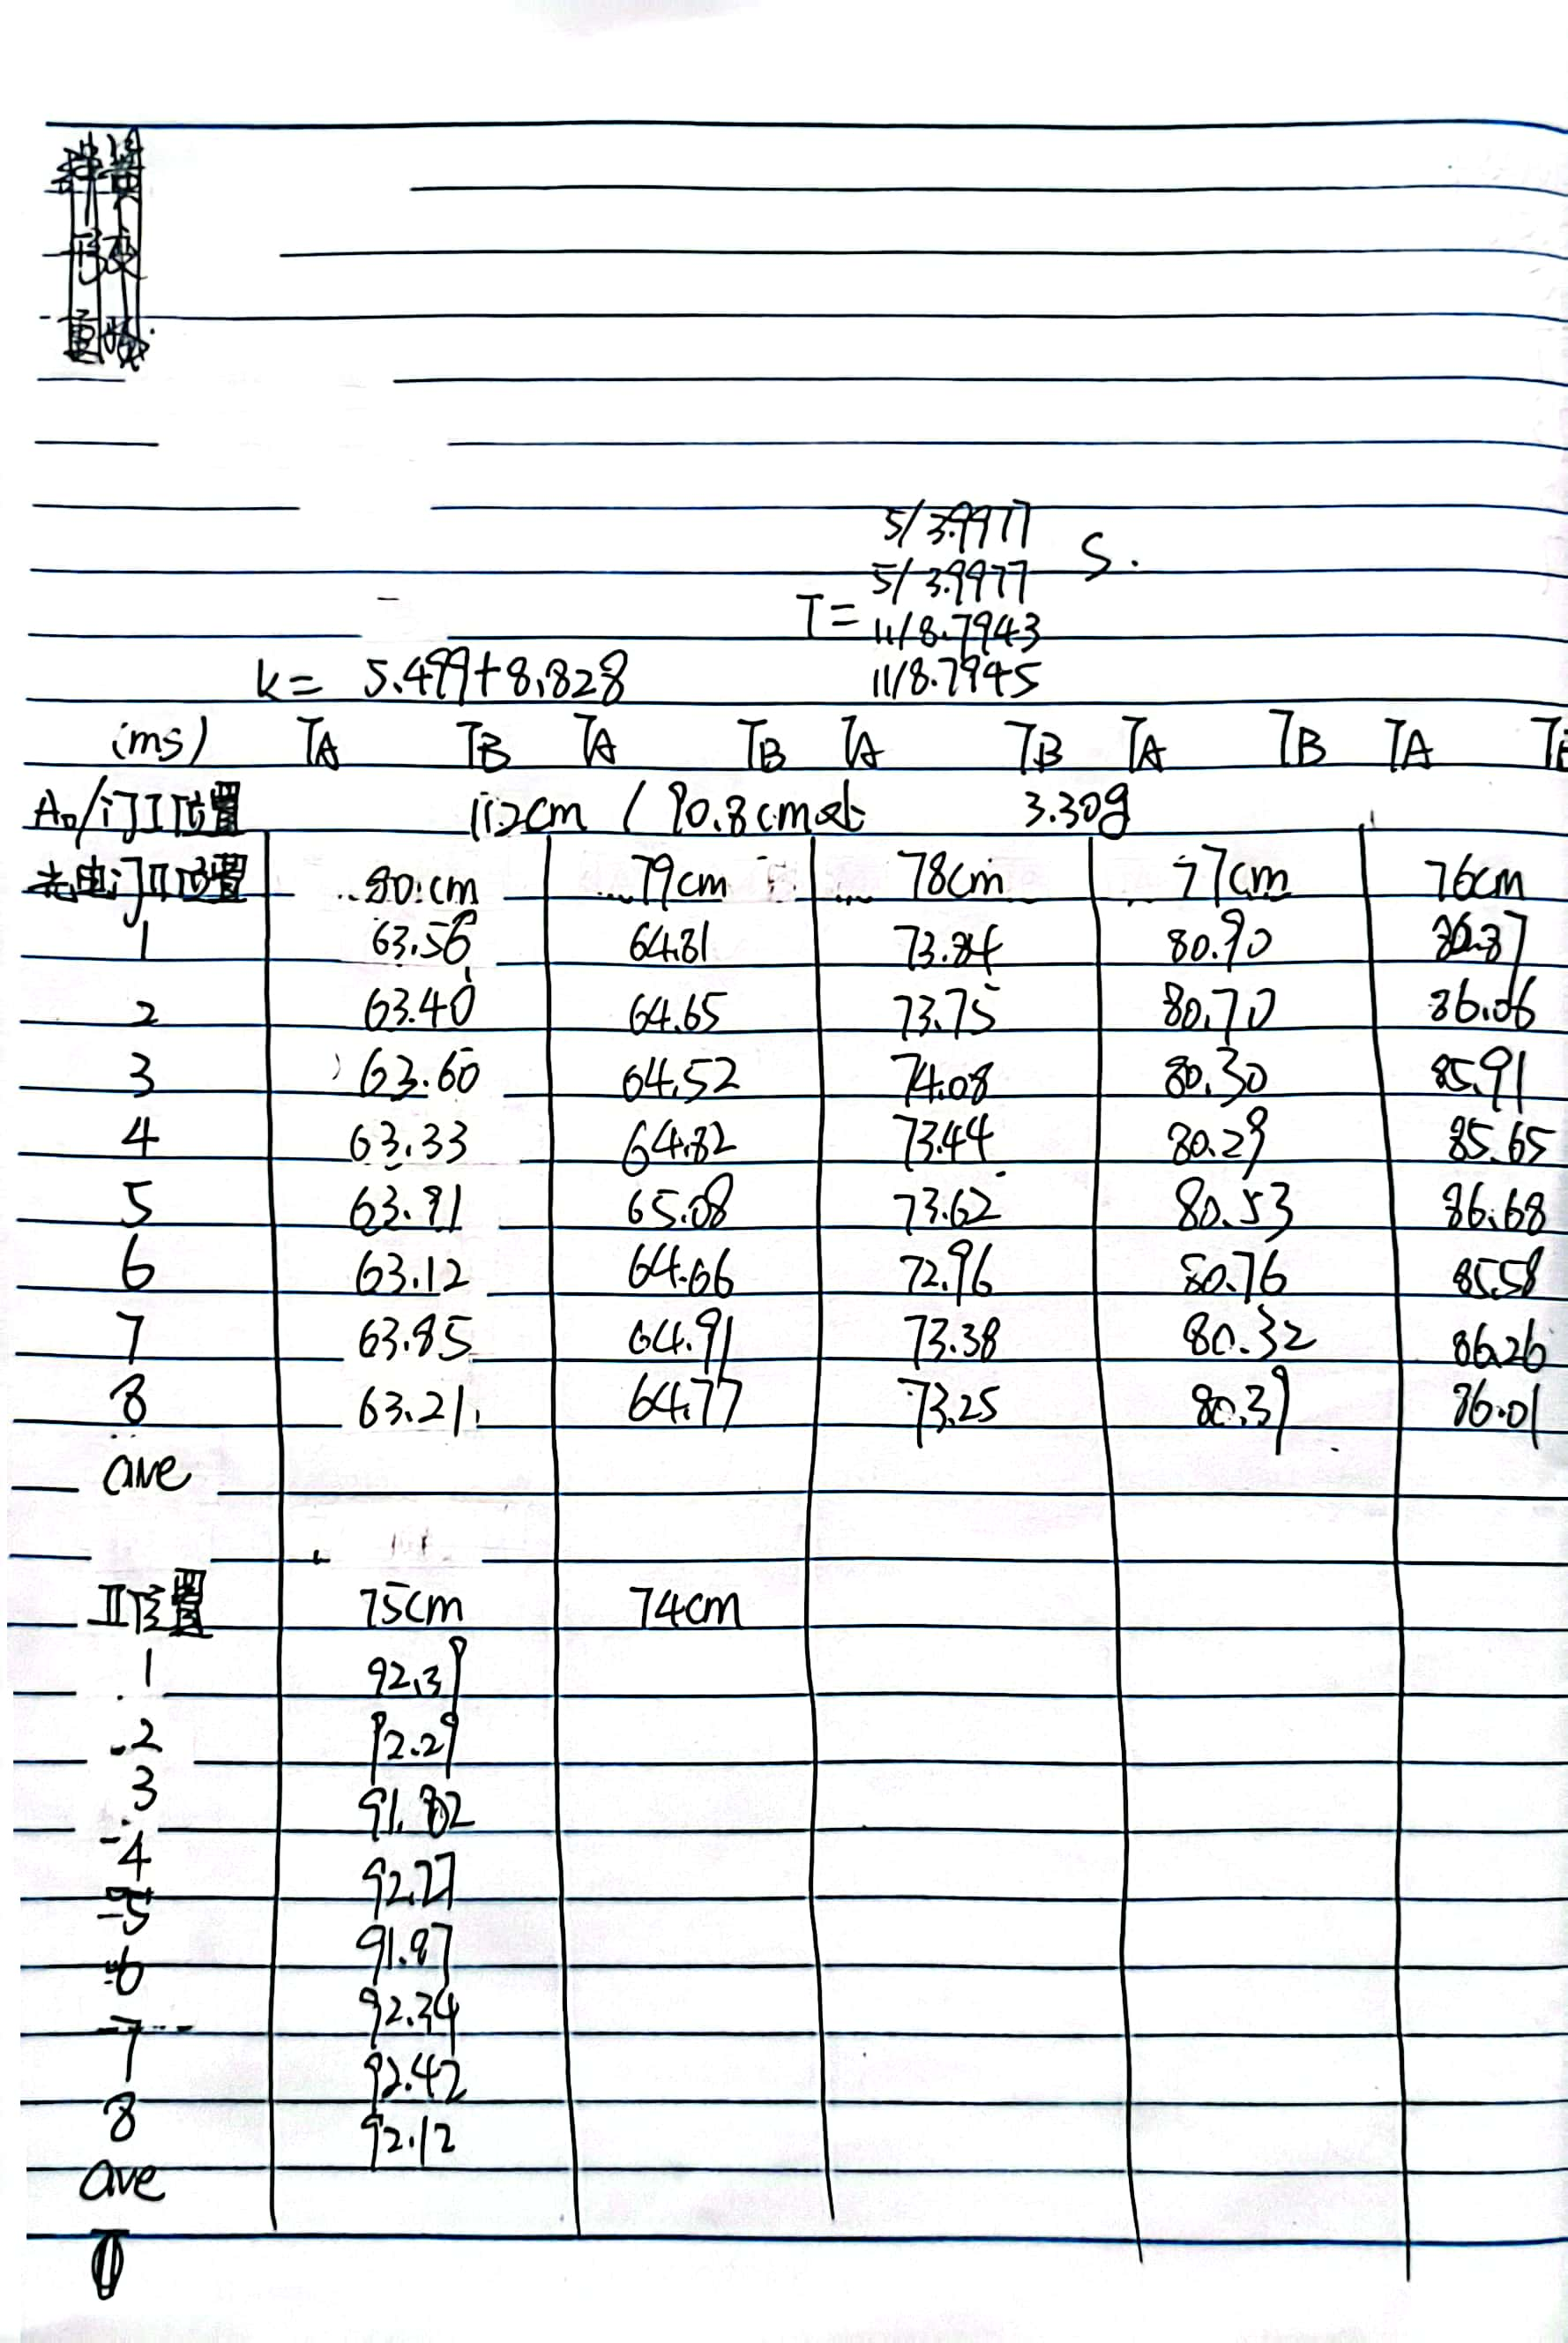
\includegraphics[height=1\textwidth,width=1\textwidth]{yuanshishujv2.jpg}
  \caption{实验原理辅助用图}\label{yuanshishujv2}
\end{figure}
\newpage
%----------------------------------------------------------------------------
\begin{figure}[h]
  \centering
  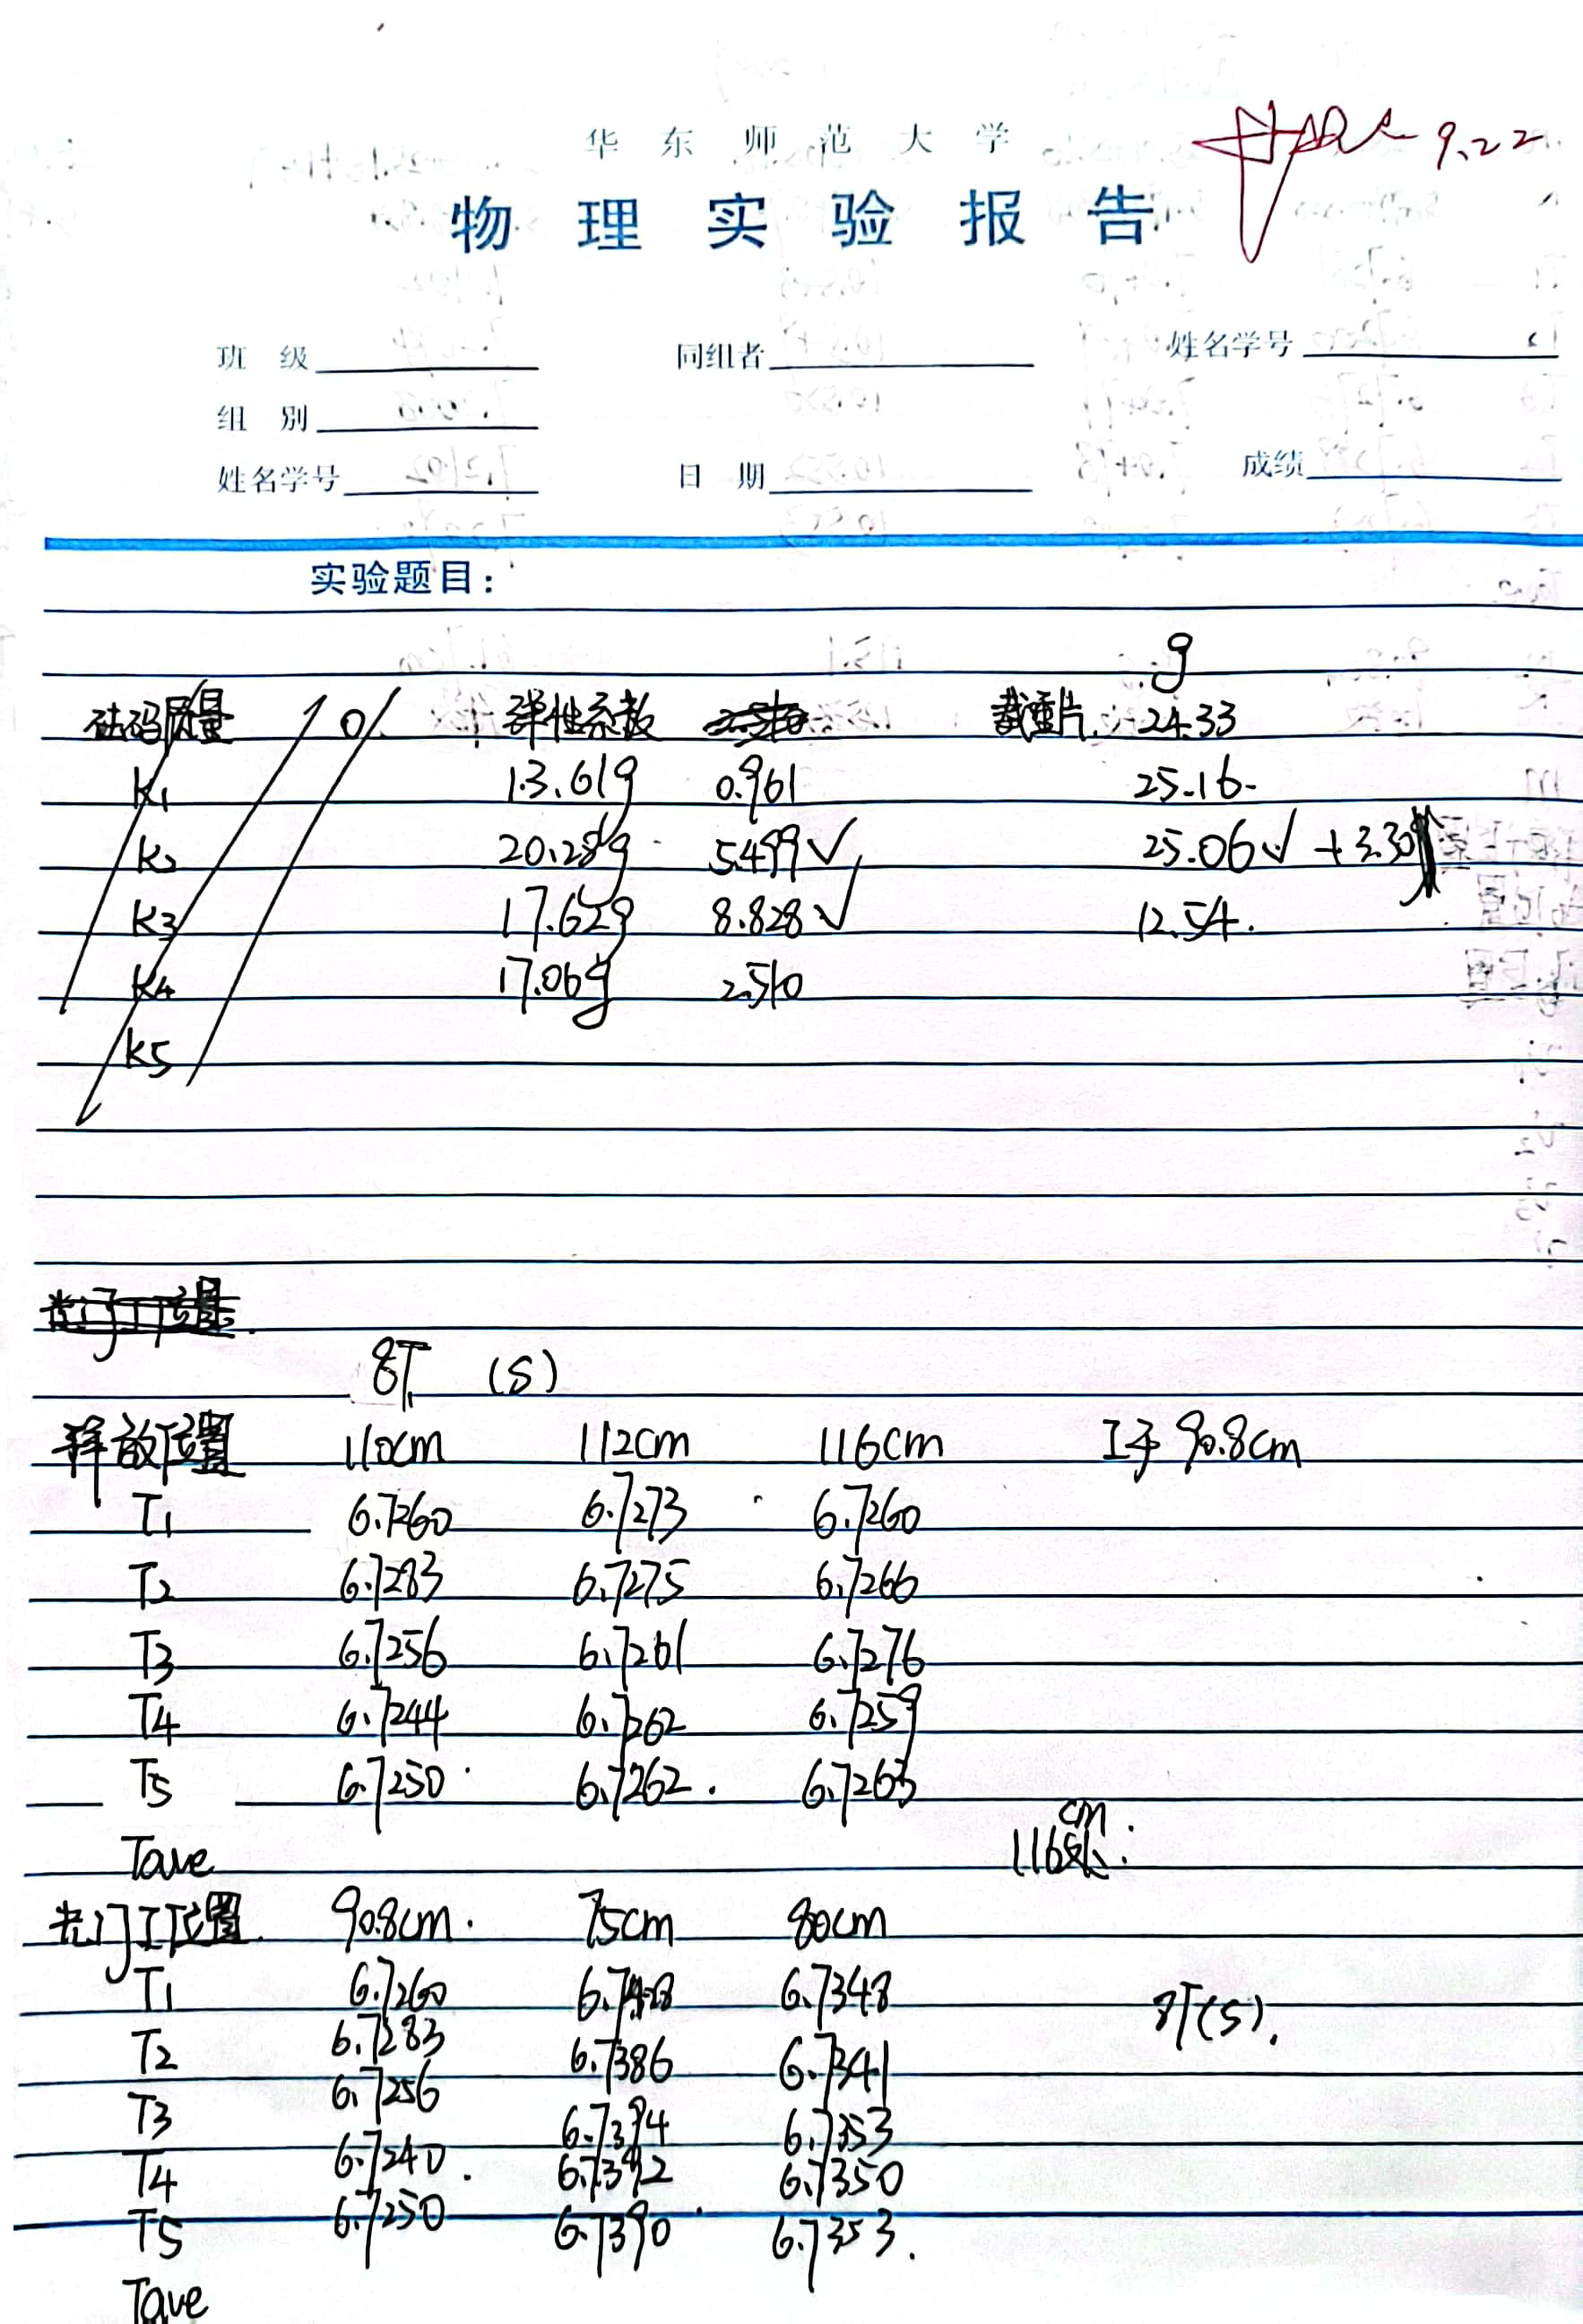
\includegraphics[height=1\textwidth,width=1\textwidth]{yuanshishujv3.jpg}
  \caption{实验原理辅助用图}\label{yuanshishujv3}
\end{figure}
\newpage

\section{实验数据处理}
弹簧质量显示如表\ref{tanhuangzhiliang}
\begin{table}[h]
  \centering   
  \caption{学生考试成绩单}\label{tanhuangzhiliang}
  \begin{tabular}{| l || l |}
      \hline
      弹性系数的弹簧 & 弹簧质量(克)\\
      \hline
      0.961 & 13.61 \\
      \hline
      5.499 & 20.28 \\
      \hline
      8.828 & 17.62 \\
      \hline
      2.510 & 17.06 \\
      \hline                       
  \end{tabular}
\end{table}
  \subsection{验证位移方程}
  \begin{figure}[b]
    \centering
    \begin{minipage}[b]{0.48\textwidth}
      \centering
      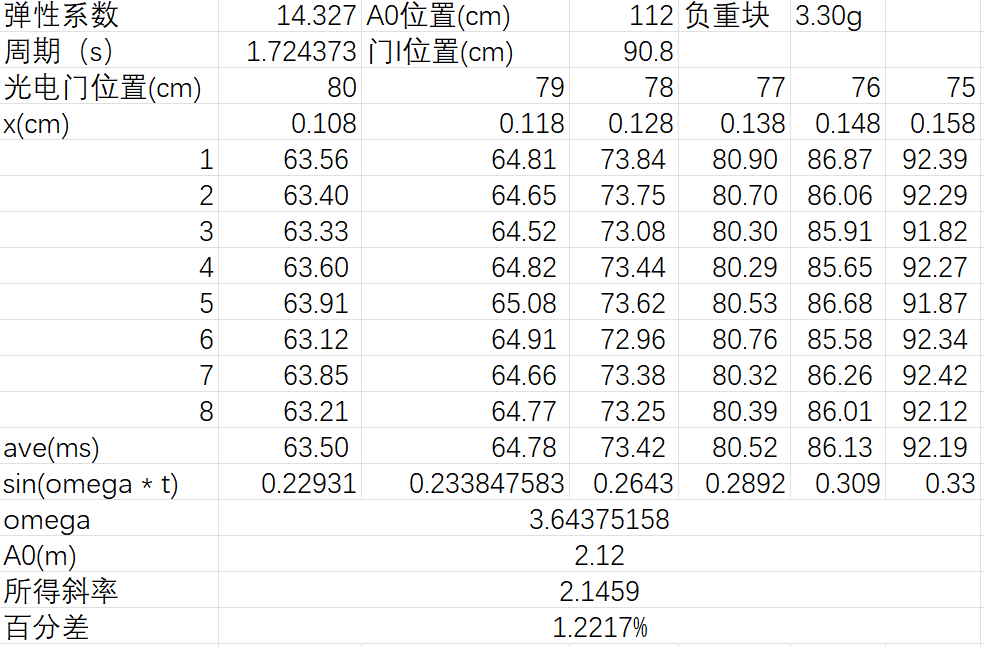
\includegraphics[width=0.46\textwidth]{yanzhengweiyifangchengshujv.png}
      \caption{验证位移方程数据}\label{yanzhengweiyifangchengshujv}
    \end{minipage}
    \begin{minipage}[b]{0.48\textwidth}
      \centering
      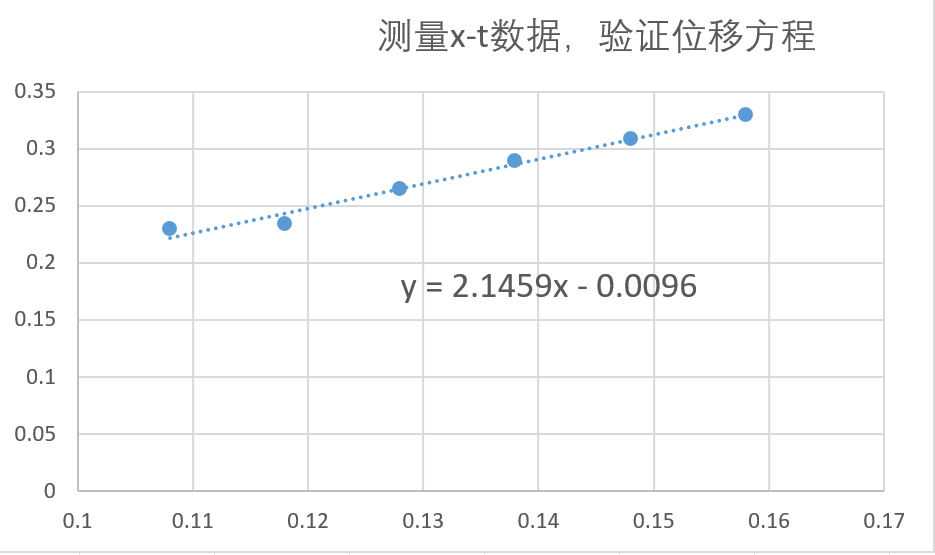
\includegraphics[width=0.46\textwidth]{yanzhengweiyifangchengzuotu.png}
      \caption{验证位移方程作图法}\label{yanzhengweiyifangchengzuotu}
    \end{minipage}
  \end{figure}

  实验数据处理如图\ref{yanzhengweiyifangchengshujv},其中计算可得实验理论$A_{0}=2.12dm$,而实验所得
  斜率,即实际测量的实际$A_{0}=2.1459dm$,两者的相差程度,即百分差为$1.2217\%$。可以证明位移方程
  $x=A\sin \left( \omega t + {\varphi}_{0} \right) \mbox{在}{\varphi}_{0} = 0 $时成立。

  实验中的误差可能来源于

  1、每次释放位置不能保证完全相同

  2、光电门传感器精度限制,以及挡光板的宽度

  3、实验中气垫滑轨不能保证完全水平,出现倾斜

  \subsection{验证振动周期与初始状态无关}
  \begin{figure}[t]
    \centering
    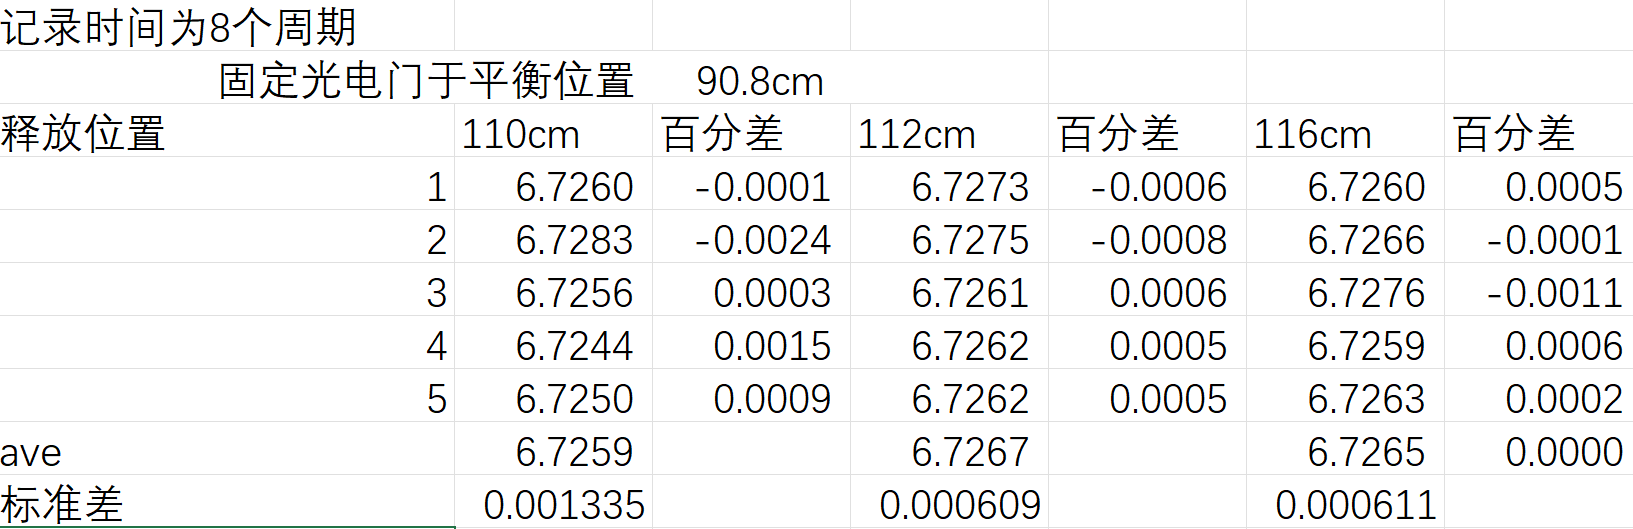
\includegraphics[height=0.3\textwidth,width=0.5\textwidth]{yanzhengwuguanshujv.png}
    \caption{验证振动周期与初始状态无关数据处理}\label{yanzhengwuguanshujv}
  \end{figure}
  验证振动周期与初始状态无关实验的数据及数据处理如图\ref{yanzhengwuguanshujv}所展示的那样。每个数据和该
  数据所在组平均值之间的相差不超过0.01s,除以八个周期后近似可以为相等,标准差也小于0.01。能验证振动周期与
  初始状态无关。

  实验中的误差可能来源于
  
  1、每次释放位置不能保证完全相同

  2、光电门传感器精度限制,以及挡光板的宽度

  3、实验中气垫滑轨不能保证完全水平,出现倾斜

  \subsection{验证周期公式$T=2\pi \sqrt{\frac{m}{k}}$}
  \begin{figure}[b]
    \centering
    \begin{minipage}[b]{0.48\textwidth}
      \centering
      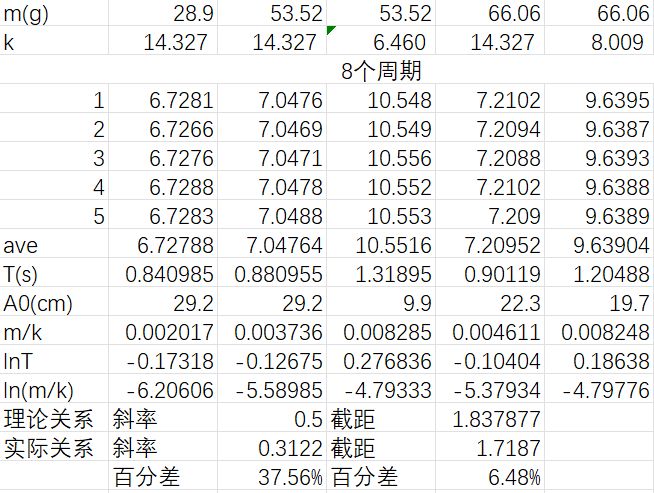
\includegraphics[width=0.46\textwidth]{yanzhengzhouqihanshu.png}
      \caption{验证周期公式$T=2\pi \sqrt{\frac{m}{k}}$实验数据}\label{yanzhengzhouqihanshu}
    \end{minipage}
    \begin{minipage}[b]{0.48\textwidth}
      \centering
      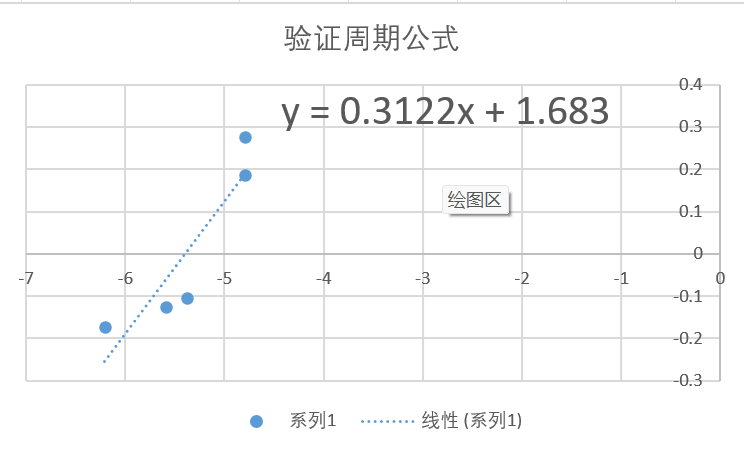
\includegraphics[width=0.46\textwidth]{yanzhengzhouqihanshuzuotu.png}
      \caption{验证周期公式$T=2\pi \sqrt{\frac{m}{k}}$数据处理}\label{yanzhengzhouqigongshizuotu}
    \end{minipage}
  \end{figure}
  验证周期公式的实验数据如图\ref{yanzhengzhouqihanshu}所示,实验数据处理如图\ref{yanzhengzhouqigongshizuotu}
  所示那样。本实验误差较大,涉及不确定度较多。
  
  实验中理论图像的斜率等于$\frac{1}{2}$,实验中理论截距为$\ln{2\pi}$。实际实验中图像的
  斜率等于$0.3122$,实际截距为$1.7187$。
  实验中理论和实际数据的百分差,斜率为$37.56\%$,截距为$6.48\%$

  实验中的误差可能来源于 
  
  1、每次释放位置不能保证完全相同

  2、光电门传感器精度限制,以及挡光板的宽度引入的误差。同时涉及质量称量,引入新的误差

  3、实验中气垫滑轨不能保证完全水平,出现倾斜

  实验中理论和实际的误差比较大,需要更多数据及更进一步的实验。其中斜率的误差较截距较大。
\newpage

\section{思考题}
  \subsection{如何开展实验探究弹簧质量对滑块振动周期的影响}
  控制滑块和载重片的质量恒定,准备若干弹簧,弹簧需要拥有相同的弹性系数但是质量不同。
  可以考虑使用不同材质做成的弹簧进行实验探究。

  将光电门I放置在平衡位置,固定初振幅,利用不同质量的的弹簧,测量在
  \begin{equation}
    \frac{\mbox{滑块总质量}}{\mbox{弹簧弹性系数}}=\frac{m}{k}=a\mbox{a为常数}
  \end{equation}
  的条件下,不同质量的弹簧测得的周期。
  
  之后通过式\ref{zhouqitanhuang}所得公式两边取对数得到
  \begin{equation}
    \ln T=\ln 2\pi + \frac{1}{2} \ln \frac{m+\frac{1}{3}m_{s}}{k}
  \end{equation}
  
  通过实验的到$\ln \frac{m+\frac{1}{3}m_{s}}{k}$和$\ln T$实验测得的值,通过作图法或者最小二乘法,求出
  斜率b和$\ln T$轴的截距,并与理论值对比,得到实验结论。
  \subsection{测量滑块在作阻尼振动时的半衰期}

  由于空气阻力的问题,滑块在气垫导轨上的运动是实际上时阻尼振动,定义阻尼振动的振幅减到初始振幅的一半时所需要的
  时间叫阻尼振动的半衰期,请设计实验,测量滑块在作阻尼振动时的半衰期。

\end{document}